\section{Reproducible numerical illustrations}
\label{sec:numerics}

The computations check explicit formulas and illustrate finite-gap
behavior. They do not estimate an unproved asymptotic exponent or
benchmark an end-to-end interior-point algorithm. The accompanying
reproduction package contains all input arrays, exact rational
certificates, scripts, raw rows including rejected points, generated
figures and tables, and a manifest of commands, software versions,
random seeds, transformations, and file hashes. Regeneration uses
Python, NumPy, SciPy, and Matplotlib without network access or imports
from another repository. High-precision scalar calculations and
reference solves use the standard-library \texttt{decimal} module.

\subsection{Exact examples}

\Cref{fig:fractional} evaluates the exact central-point and stable
quadratic-root formulas from \cref{thm:fractional-spectrum} with 80 decimal digits,
for $g=10^{-2},10^{-3},\ldots,10^{-24}$. Dividing the four scaled
eigenvalues by their proved limits displays convergence to one.
The paired section retains the two $(b,g)$ eigenvalues and consequently
has a different condition-number exponent. At $g=10^{-2},10^{-4},10^{-6}$,
a separate float64 computation forms the Hessian through
$\tr(X^{-1}UX^{-1}V)$ and solves the generalized eigenproblem using
the tangent Gram matrix. Its eigenvalues agree with the scalar formulas
to relative error below $10^{-7}$. The high-precision formulas avoid
subtracting nearly equal quadratic roots by obtaining the smaller root
from the determinant divided by the larger root.

\begin{figure}[tb]
\centering
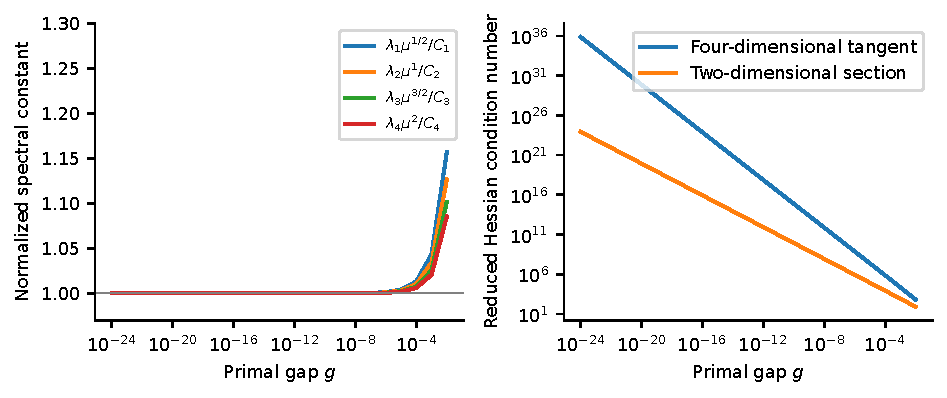
\includegraphics[width=\textwidth]{figures/fractional-sdp.pdf}
\caption{The fractional SDP and its section. Left: the scaled ordered
eigenvalues divided by $C=(\sqrt2,1,\sqrt2,4/7)$, with powers
$(1/2,1,3/2,2)$ of $\mu$. Right: the condition numbers on the two
tangent spaces. Both optimality systems have singularity degree two.}
\label{fig:fractional}
\end{figure}

For the simplex of \cref{prop:simplex-plateau}, the exact log-barrier
center satisfies $x_i=\mu/(c_i+z)$, where $z>0$ is the unique root of
$\sum_i\mu/(c_i+z)=1$. We solve this scalar monotone equation with
70 decimal digits and evaluate the Hessian through its factor.
\Cref{fig:lp-numerics} shows the inverse-square regime giving way to the large limiting
plateau when $g$ falls below $\vartheta$.
For the compact degenerate LP of \cref{ex:degenerate-lp}, direct centering
gives, at $\mu=10^{-9}$,
$\mu^2\lambda_{\min}\approx0.24888160$ and
$\mu^2\lambda_{\max}\approx1.14289068$, consistent with the proved
limit and $\kappa(L)\approx4.59210571$. The full sequence and its
centrality residuals are supplied in the data package.

\begin{figure}[tb]
\centering
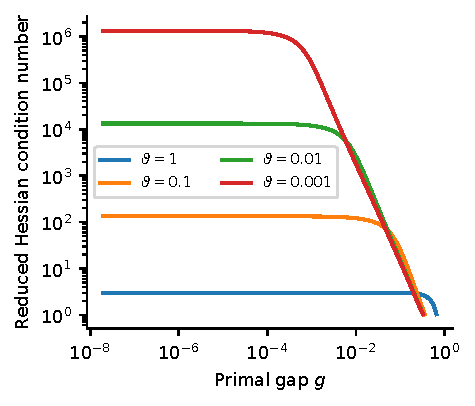
\includegraphics[width=.49\textwidth]{figures/simplex-plateau.pdf}\hfill
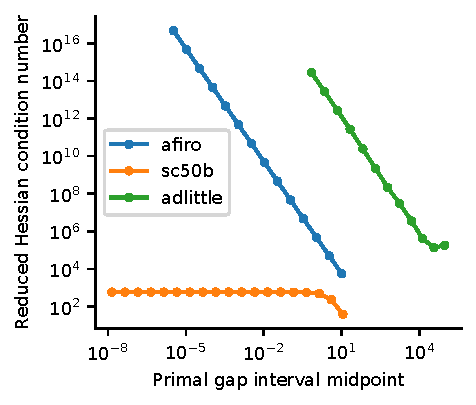
\includegraphics[width=.49\textwidth]{figures/netlib.pdf}
\caption{Left: near-degenerate simplex plateaus for fixed values of
$\vartheta$. Right: accepted finite-gap points for the frozen Netlib
representations. The latter curves are numerical observations; no
asymptotic exponent is fitted to them.}
\label{fig:lp-numerics}
\end{figure}

\Cref{tab:oscillatory} evaluates the exact subsequence in
\cref{prop:oscillatory-barrier}. It records the norm of the discarded
forcing component divided by $g$, and the relative Euclidean error
of the solution obtained by retaining only the strong eigenmode.
The forcing component tends to zero at the proved rate while the
solution error tends to one. This is a direct check of the distinct
residual and solution contracts, not an iterative-solver artifact.

\begin{table}[tb]
\centering
\begin{tabular}{rrrr}
\toprule
$k$ & $g_k$ & $\|\Pi c\|/(g_k\|c\|)$ & Relative solution error\\
\midrule
1 & 1.87e-03 & 0.01000003 & 0.93680040 \\
2 & 3.49e-06 & 0.01000000 & 0.99999976 \\
3 & 6.51e-09 & 0.01000000 & 1.00000000 \\
4 & 1.22e-11 & 0.01000000 & 1.00000000 \\
\bottomrule
\end{tabular}

\caption{Oscillatory barrier with $\epsilon=0.01$ and
$g_k=\exp(-2\pi k)$. The relative solution error is
$\|H^{-1}\Pi c\|/\|H^{-1}c\|$. Rounded values of one do not assert
exact equality at finite gap.}
\label{tab:oscillatory}
\end{table}

\subsection{Certified benchmark representations and precision screens}

We use three small Netlib LPs \citep{netlib}: \texttt{afiro},
\texttt{sc50b}, and \texttt{adlittle}. The frozen arrays are the result
of HiGHS 1.15.1 default presolve followed by conversion of inequalities
and finite bounds to equality constraints and nonnegative variables.
Their dimensions, from original MPS to presolved model to standard form,
are respectively
$(27,32)\to(7,10)\to(9,18)$,
$(50,48)\to(15,15)\to(15,29)$, and
$(56,97)\to(53,95)\to(55,136)$.
The Hessian uses the Euclidean metric in these final coordinates.
It is not the Hessian of the original MPS representation. The frozen
arrays define the tested instances, so a later presolver version is
not needed for reproduction.

The hypotheses are checked without feasibility tolerances. Every
stored float64 input is interpreted as its exact binary rational.
The package verifies a rational point $x>0$ with $Ax=b$ and a rational
vector $y$ with
\[
 A^\top y+\eta c>0,\qquad \eta\geq0.
\]
For $x\geq0$ in a fixed upper objective sublevel,
$x^\top(A^\top y+\eta c)=b^\top y+\eta c^\top x$ bounds every
coordinate. The certificates use $\eta=0$ for \texttt{afiro} and
\texttt{sc50b}, proving compactness of their feasible sets, and
$\eta=1$ for \texttt{adlittle}, proving compactness of its objective
sublevels. Thus the localized theorem applies to the last instance.
Rational primal and dual feasible points also certify brackets on the
optimal value, with widths approximately $8.2\cdot10^{-12}$,
$9.4\cdot10^{-12}$, and $4.5\cdot10^{-7}$, respectively.

Centering uses an orthonormal nullspace basis $W$ and the Hessian factor
$B=\Diag(x^{-1})W$. Singular values of $B$ give the Hessian eigenvalues
by squaring; Newton solves and decrements use the same factorization.
Each stored iterate is repaired to an exactly feasible rational point
using a fixed nonsingular column basis. We evaluate its objective
exactly and subtract the certified optimal-value bracket. A point is
accepted for the plot only when this gap interval is positive and
has relative width at most $1\%$, the repaired point is positive,
the maximum relative coordinate repair is at most $10^{-4}$, the
scaled equality residual is at most $10^{-12}$, and the \emph{unscaled}
centrality decrement is at most $10^{-5}$. We additionally require
\[
 \epsilon_{\rm mach}\max(n,d)\,\kappa_2(B)\leq10^{-6}.
\]
This last screen is a numerical resolution indicator for the factor
SVD, not a rigorous interval certificate for its singular values.
The exact rational certificates establish the instance hypotheses;
the plotted spectral values remain finite-precision computations.

\begin{table}[tb]
\centering
\begin{tabular}{lrrrrr}
\toprule
Instance & $(m,n)$ & Accepted/attempted & Last gap & $\kappa$ & $\rho$\\
\midrule
afiro & $(9,18)$ & 14/27 & 3.34e-06 & 4.65e+16 & 2.2e-07 \\
sc50b & $(15,29)$ & 19/27 & 1.40e-08 & 5.82e+02 & 6.1e-07 \\
adlittle & $(55,136)$ & 12/27 & 6.80e-01 & 2.81e+14 & 2.5e-09 \\
\bottomrule
\end{tabular}

\caption{Accepted Netlib points and the last accepted point in each
continuation sequence. All 27 attempted points per instance, including
centrality, gap, repair, or spectral-resolution rejections, are retained
in the raw data.}
\label{tab:netlib}
\end{table}

\Cref{tab:netlib} makes the different resolved accuracy ranges explicit.
In particular, the stringent spectral screen stops \texttt{adlittle}
well before its deepest attempted gap. We draw no conclusion about
its limiting condition number from that truncation. The near-degenerate
simplex already proves why a finite observed slope or plateau should
not by itself be treated as an asymptotic classification.

\subsection{Clustered CG and the meaning of stopping accuracy}

To exercise two intervals with many distinct eigenvalues, we generate a
$60\times60$ symmetric matrix from a fixed-seed orthogonal rotation of
30 equally spaced values in $[1,2]$ and 30 in $[g^{-2},3g^{-2}]$.
This is a synthetic spectral test, not a claimed Newton Hessian.
The actual float64 matrix is explicitly symmetrized. CG uses ordinary
float64 matrix-vector products and stops when its recursively updated
relative residual first reaches $10^{-8}$. At that iterate, an 80-digit
solve of the exact real system defined by the stored float64 matrix
and right-hand side supplies the reference solution, relative energy
error, and independently evaluated true residual.

\begin{table}[tb]
\centering
\begin{tabular}{rrrrr}
\toprule
$g$ & Iterations & Recursive residual & True residual & Relative energy error\\
\midrule
1e-01 & 43 & 8.82e-09 & 8.82e-09 & 3.54e-09 \\
1e-02 & 71 & 2.56e-09 & 2.56e-09 & 4.21e-09 \\
1e-03 & 96 & 4.37e-09 & 4.39e-09 & 4.24e-09 \\
1e-04 & 124 & 2.95e-09 & 2.52e-08 & 8.55e-09 \\
\bottomrule
\end{tabular}

\caption{Float64 CG on the synthetic two-interval matrices. The final
two columns use an 80-digit reference calculation for the actual rounded
matrix and right-hand side. The last recursive stopping test does not
certify a true relative residual below $10^{-8}$.}
\label{tab:cg}
\end{table}

The prescribed internal interval ratios are two and three while the
interval separation grows; these ratios precede floating-point matrix
construction and are not exact spectral assertions for the rounded
matrix. \Cref{tab:cg} illustrates the benefit of this structure
and the distinction between stopping metrics. It is not an empirical
proof of the exact-arithmetic degree bound. Indeed, exact-arithmetic
CG terminates in at most 60 steps for these matrices, whereas floating
arithmetic can take more steps because conjugacy is lost. Recomputed
residuals and energy error therefore remain separate reported quantities,
as required by the solver contract in \cref{sec:clustered-solves}.
